\chapter{関連研究}
\label{chap:relatedResearch}

本章では関連研究を紹介し、それらの特徴や本研究との関連性について示す。

\newpage


\section{主要な研究領域}
本研究ではNFCのタッチインタラクション及びwikiベースなARナビゲーションが有用であることを検討した。
本研究に関連する先行研究は大きく以下のように分類できる
\begin{itemize}
  \item ARをナビゲーションに利用する研究
  \item ユーザの位置測位及びコンテキスト情報の取得に関する研究
  \item NFCを用いて情報を取得し、ナビゲーションに応用する研究
  \item AR情報の整理・関連情報推薦にハイパーリンクを利用する研究
\end{itemize}
それぞれについて関連性の高いものを紹介した上で本研究との関連性を示す。

\section{ARをナビゲーションに利用する研究}
ARを地理情報のナビゲーションとして利用する代表的な研究及びシステムを紹介する。

\subsection{A Touring Machine}
Feinerらが開発したA Touring Machine\cite{629922}はヘッドマウント・ディスプレイとスタライスで操作可能な2Dディスプレイで大学のキャンパスの情報を表示するアプリケーションであり、ARを利用した地理情報ナビゲーションの初期研究として挙げられる。
このシステムではGPSによる位置情報と磁気センサによる向きの情報からユーザの位置と向きを推定し、ヘッドマウント・ディスプレイに大学の情報が表示される(図\ref{fig:a_touring_machine_ar})。
また手持ちのスタライスで操作可能な2Dディスプレイが専用のHTTPサーバにつながっており、表示したい情報のリンクに触れるなどの操作をすることでヘッドマウント・ディスプレイでの表示情報が変化する。
ナビゲーションでの表示やシステム構成などが現在のARナビゲーションアプリに通ずる一方で、GPSと磁気センサによる位置測位には精度の面で課題があった。
また当時の技術ではヘッドマウント・ディスプレイとコンピュータを小型化することが難しかったため、図\ref{fig:a_touring_machine_pc}のように装備が大きく、屋外で常用することは現実的でなかった。

\begin{figure}[h]
  \begin{minipage}{0.5\hsize}
    \centering 
    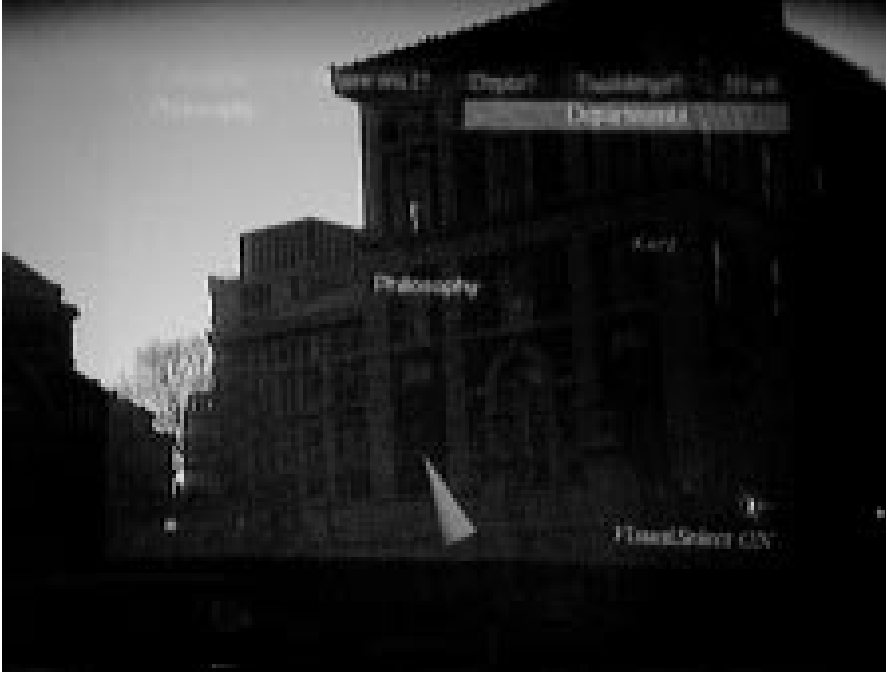
\includegraphics[height=60mm]{images/a_touring_machine_ar.png}
    \caption{表示されたキャンパスの情報} \label{fig:a_touring_machine_ar}
  \end{minipage}
  \begin{minipage}{0.5\hsize}
    \centering 
    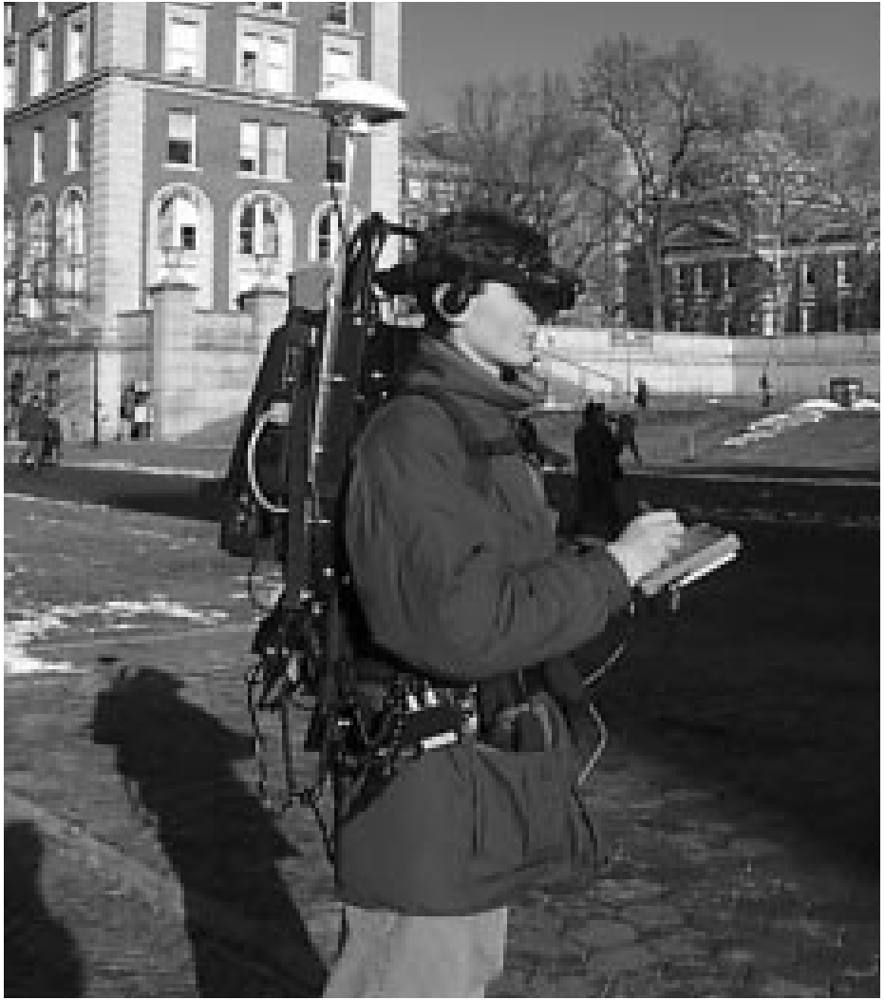
\includegraphics[height=60mm]{images/a_touring_machine_pc.png}
    \caption{実際の装備} \label{fig:a_touring_machine_pc}
  \end{minipage}
\end{figure}


\subsection{KARMA}
FeinerらがKnowledge-based augmented reality\cite{10.1145/159544.159587}で提案したKARMAはレーザープリンターのメンテナンスをARで説明するプロトタイプシステムである。
図\ref{fig:karma}のようにヘッドマウント・ディスプレイによってレーザープリンターの内部機構に関する情報を提示し、ユーザがメンテナンスするときの理解を助けるシステムである。
位置測位には超音波センサを利用しており、正確な位置測位と情報の投影が可能である。
一方で高価で大型な超音波センサをすべての対象に取り付ける必要があり、現実的に利用するにはより良い測位システムを利用する必要があった。

\begin{figure}[h]
  \centering
  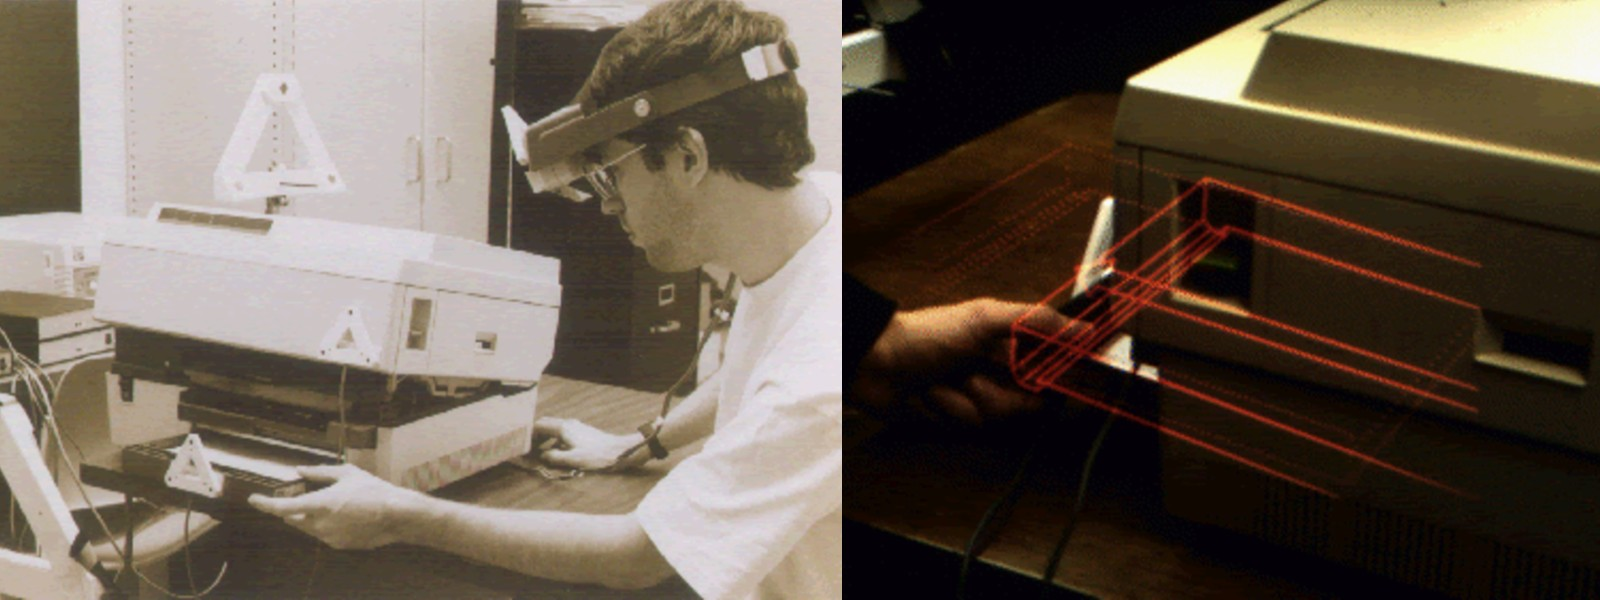
\includegraphics[width=150mm]{images/karma.jpg}
  \caption{KARMA} \label{fig:karma}
\end{figure}


\subsection{MARS}
HöllererらによるMARS\cite{MARS}は上記の「A Touring Machine」及び「KARMA」の方式を組み合わせ、屋外でのARナビゲーションと室内でのARによる地図操作を結びつけたシステムである。
ユーザは屋外でこのシステムを利用することでヘッドマウントディスプレイを通して建物に重ねて表示されたナビゲーションを見ることができる(図\ref{fig:mars_ar})。またPC上で作成された経路情報を実際の景色に投影することも可能である(図\ref{fig:mars_route})。
一方で屋内ではMARSを利用することで、机の平面上に仮想の地図が投影される。この仮想地図はトラックボールや位置センサの搭載されたオブジェクトを利用することで操作でき、屋外のユーザが見ている経路情報などを編集することができる(図\ref{fig:mars_ar_indoor})。
このように屋外でのナビゲーションを編集する環境として屋内でのAR環境を利用し、屋内と屋外のARビューに相互作用をもたせる方式はユーザのAR情報編集の体験向上に大きく寄与すると思われる。
このような編集環境の状態がインタラクティブにARでの情報に作用するという点は本研究とも関連があると言える。

\begin{figure}[h]
  \begin{minipage}{0.5\hsize}
    \centering 
    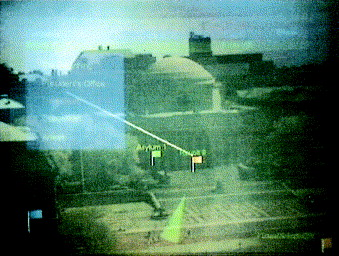
\includegraphics[height=60mm]{images/mars_ar.png}
    \caption{ARでの表示} \label{fig:mars_ar}
  \end{minipage}
  \begin{minipage}{0.5\hsize}
    \centering 
    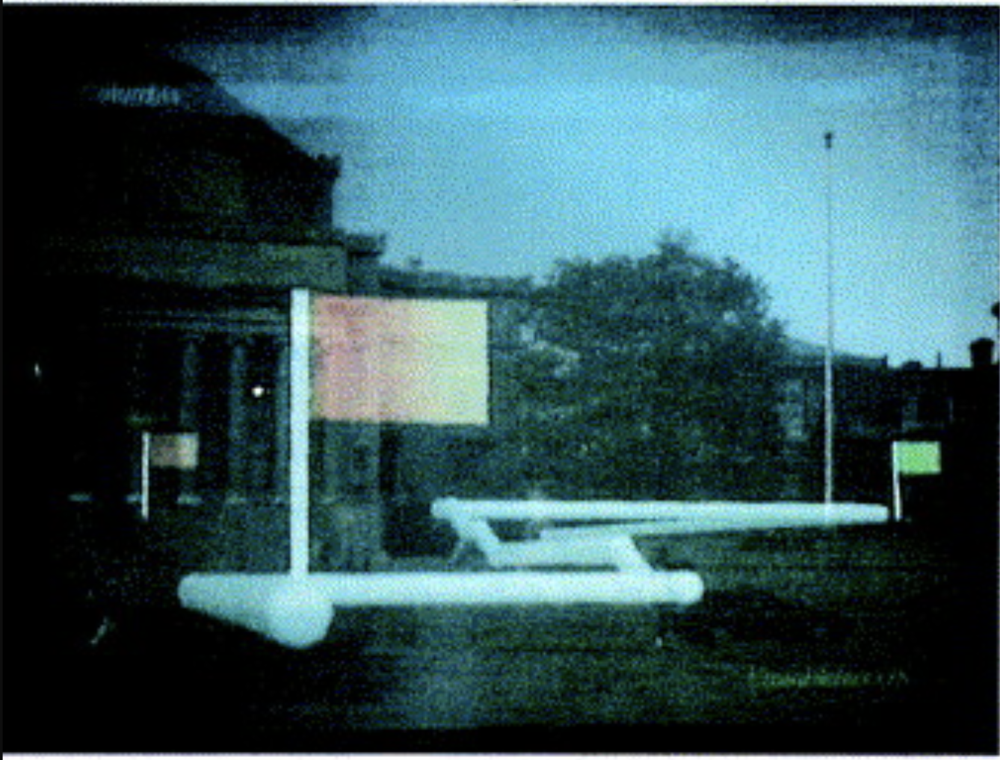
\includegraphics[height=60mm]{images/mars_route.png}
    \caption{経路の投影} \label{fig:mars_route}
  \end{minipage}
\end{figure}


\begin{figure}[h]
  \centering
  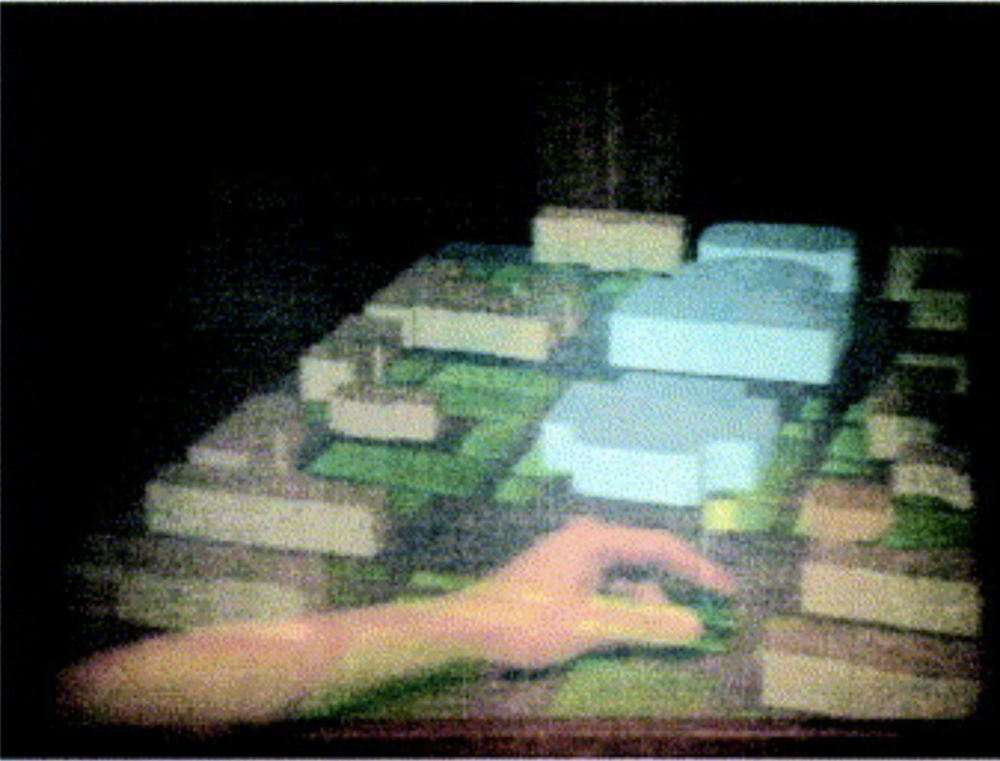
\includegraphics[height=60mm]{images/mars_ar_indoor.png}
  \caption{屋内での利用} \label{fig:mars_ar_indoor}
\end{figure}

\subsection{NaviCam}
暦本らによるNaviCam\cite{10.1145/215585.215639}はマーカーをカメラで認識し、マーカー応じてその場に即した説明を手持ちの2Dディスプレイやヘッドマウントディスプレイに提示するシステムである。
現在主流になっているマーカーベースのARの初期研究であり、青と赤の線で構成されたカラーコードと呼ばれるバーコードを認識することで状況と対象物の位置を把握し、情報を提示している。
カラーコードの画像認識からARを表示するこの方式は前述のような超音波センサを利用する方式などと比べ圧倒的に低コストであり、カラーコード上での表示は正確であるため屋内での位置測位に有利であると言える。
またコードのパターンによりコンテキスト情報を埋め込むことが可能である点も既存の測位システムにない特徴であった。

\begin{figure}[h]
  \centering
  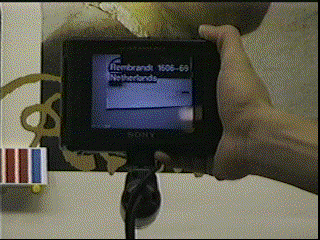
\includegraphics[height=70mm]{images/NaviCam.png}
  \caption{NaviCam} \label{fig:NaviCam}
\end{figure}


\subsection{Feature-Based Indoor Navigation Using Augmented Reality}
KasprzakらはFeature-Based Indoor Navigation Using Augmented Reality\cite{6597797}で室内での利用を想定したモバイル端末のARナビゲーションのプロトタイプを作成し評価している。
このプロトタイプは画像として登録された特徴的なアイコンなどを元に画像認識(図\ref{fig:FBINUAR_image})から位置情報と向きを推定し、ユーザの目的地を矢印で表示する(図\ref{fig:FBINUAR_ar})ものである。
またこのプロトタイプを利用し、実際に建物内での案内に利用するテストを行っている。
その結果2Dの地図と比べて目的地までの到達時間が短縮され、被験者が立ち止まったり間違えた方向に進む回数も減少したと報告している。
室内での利用を視野に入れている点はGPSなどを利用するシステムと違い、本研究に近いが登録した画像による位置推定には以下のような課題もある。
\begin{itemize}
  \item 特徴的なロゴやアイコンの無いところでは登録できる画像がなく精度が保証できない
  \item 各場所で個別に画像の登録が必要
  \item 距離や明るさなどによっては認識できない可能性がある
\end{itemize}
またこのプロトタイプシステムでは事前に選択した目的地に正確に早く到着することに主眼を置いており、本システムのようにハイパーリンクによる関連情報から周辺譲歩を探索する用途を考えていない点も本研究との違いである。

\begin{figure}[h]
  \centering 
  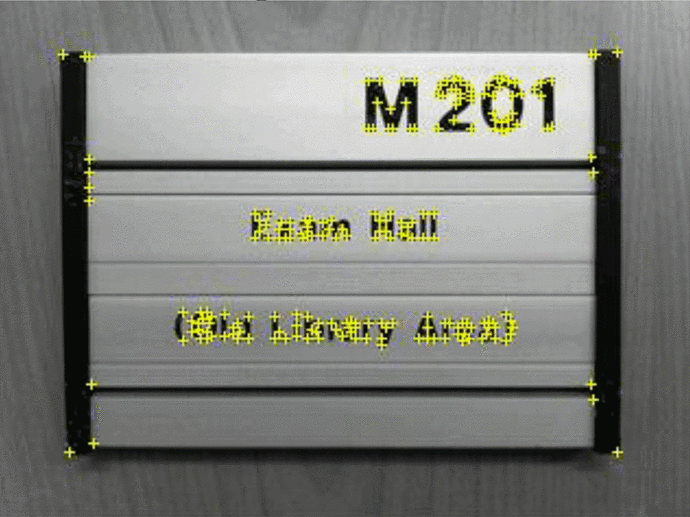
\includegraphics[height=70mm]{images/FBINUAR_image.png}
  \caption{特徴量による画像認識} \label{fig:FBINUAR_image}
\end{figure}
\begin{figure}[h]
  \centering 
  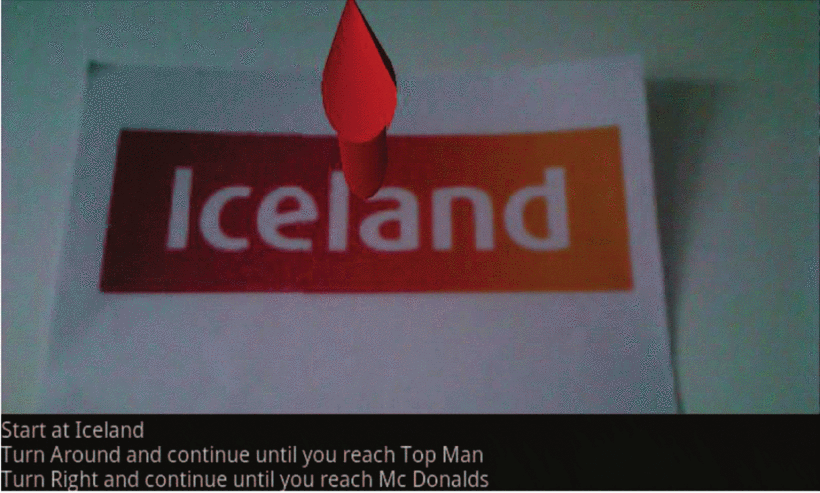
\includegraphics[height=70mm]{images/FBINUAR_ar.png}
  \caption{矢印による案内} \label{fig:FBINUAR_ar}
\end{figure}


\subsection{Wikitude}
Wikitude(図\ref{fig:Wikitude})は、Wikitude GmbH\footnote{\textsf{TODO:todo}}が開発したモバイル向けARソフトウェアである。
モバイル端末のGPSと磁気センサ、加速度計からユーザの位置と向きを推測し周囲情報をディスプレイに表示する。
コンテンツの追加にはKMLやARML(Augmented Reality Markup Language)と呼ばれるXML互換のフォーマットが使われている。
KMLはGoogleMapなどが対応した地理空間情報の情報記述を目的としたXML互換のファイル形式であり、ARMLはKMLを更に拡張したファイル形式である。
KMLファイルはGoogleMapでの読み込みや作成が可能でありユーザはGoogleMapからAR情報を作成できる。
一方でGPSと磁気センサによる位置推定には精度の面で課題があるだけでなく、GPSの利用できない屋内などでは利用できない欠点がある。
またARでの情報登録する際にGoogleMapなどの地図アプリケーションから作成するかKMLファイルを自身で編集する必要があり、本システムとは以下のような点で異なっている。
\begin{itemize}
  \item 共同編集が難しい
  \item 編集環境がWYSIWYGでない
  \item AR情報同士のハイパーリンクを記述するのが難しい
\end{itemize}

\begin{figure}[h]
  \centering 
  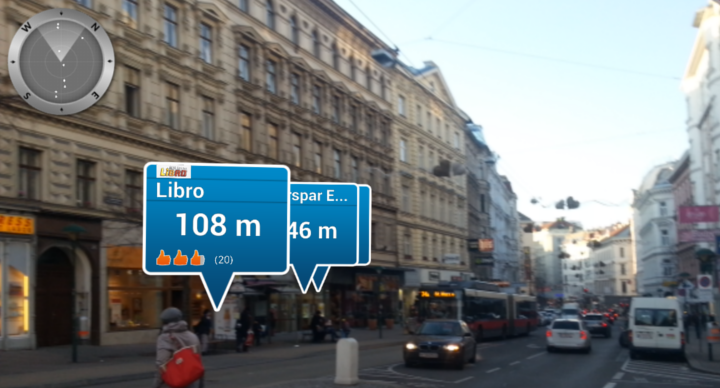
\includegraphics[width=120mm]{images/Wikitude.png}
  \caption{Wikitude} \label{fig:Wikitude}
\end{figure}



\section{ユーザの位置測位及びコンテキスト情報の取得に関する研究}
前節でも挙げたとおりARによるナビゲーションではユーザ位置測位やコンテキスト情報取得には様々な方式が検討されている。
前節に挙げたARナビゲーションシステムでは検討されなかった位置測位システム及びそれらを比較する研究を紹介する。
さらにこれらの測位を複合的に扱いコンテキスト把握につなげるシステムも紹介する。

\subsection{RSSI based Bluetooth low energy indoor positioning}
JianyongらによるRSSI based Bluetooth low energy indoor positioning\cite{7275525}ではBluetooth Low Energy\footnote{\textsf{TODO:todo}}による位置測位が提案されている。
複数の送信機から送られたBluetoothの電波のRSSI(Received Signal Strength Indicator:受信信号強度)を元に位置測位を行うものである。
Bluetoothは現在普及しているモバイル端末のほぼ全てが対応する通信形式であり、Bluetooth Low Energyは使用電力も少なくて済むという利点がある。
一方で複雑な形状の空間や遮蔽物がある場所では測位が難しいという難点があり、正確な測位のためには多くのサンプリングが必要になる。
またGPSやNFCタグなどと比べると一定範囲ごとにBluetoothの送信機が必要になりコストも高いというデメリットがある。


\subsection{Recent Advances in Wireless Indoor Localization Techniques and System}
FaridらによるRecent Advances in Wireless Indoor Localization Techniques and System\cite{Farid2013}では屋内でのユーザの位置測位手法の分析が行われている(図\ref{fig:IndoorLocalization})。
この研究では多くの方式について比較を行っているが、モバイル端末自体以外に特殊な装置を必要としないことを条件にするとGPS、Wifi、Bluetoothの3つに絞られる。
それぞれに対して位置測位の面で以下のような特徴があるとしている。
\begin{itemize} 
  \item GPS\\
    屋外では利用できるが屋内では利用できず、精度も6~10mと良いとは言えない。また位置の取得までに多少の時間がかかるという難点があるとしている。
  \item Wifi\\
    屋内屋外を問わず問わず1~5mの精度で測位できるが、消費電力が高く設置コストが高いという難点がある。
  \item Bluetooth\\
    カバーする範囲が狭く屋内での利用に限られるが消費電力が少なく、2~5mの精度で測位ができる。一方で設備コストが高いことが難点である。
\end{itemize}
このようにモバイル端末で位置測位を行う方式は複数あるが、どれも精度やコストの面で難点がある。
一方本研究で提案したNFCタグによる位置測位はユーザがNFCタグにタッチしなくてはならない点を除くと低コストで正確な位置測位が可能である。
位置測位以外にもNFCタグにコンテキスト情報の結びつけが行える点やタグにタッチするだけでアプリの起動を行えることを踏まえれば十分に有用であると言える。

\begin{figure}[h]
  \centering 
  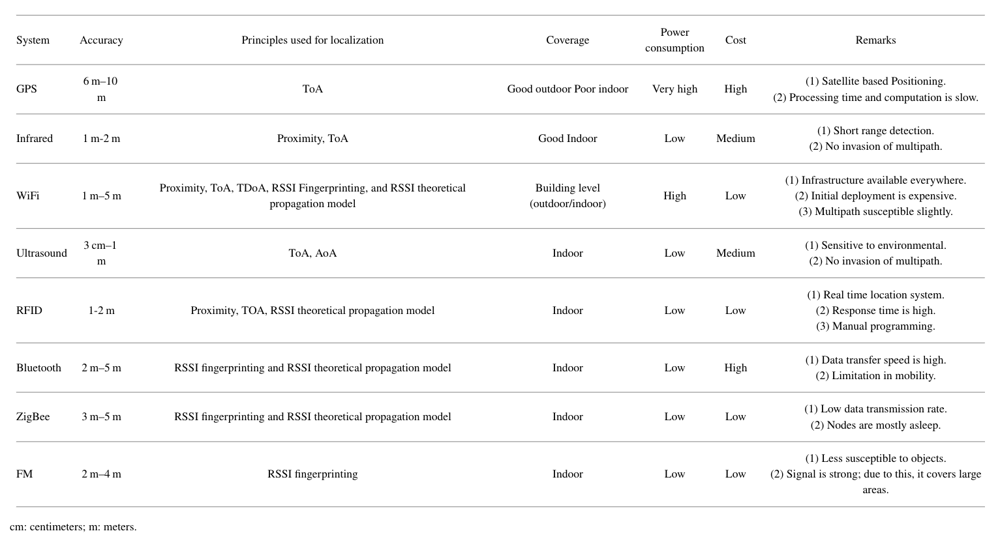
\includegraphics[width=120mm]{images/IndoorLocalization.png}
  \caption{屋内での位置測位手法の比較} \label{fig:IndoorLocalization}
\end{figure}


\subsection{App Clips}
App Clips\footnote{\textsf{https://developer.apple.com/documentation/app\_clips}}はApple\footnote{\textsf{TODO:todo}}が2020年にiOS向けに発表した機能である。
App ClipsはNFCタグやQRコードの読み込みや位置情報をトリガにして決済、情報提示等を行う仕組みである。
専用のNFCタグやQRコードを読み込んだり、GPSからの情報で特定の位置にいたりすると登録された小規模アプリケーションがインストールなしに利用できる(図\ref{fig:appClips})。
これは上記のようなユーザの位置測位システムを統合しコンテキスト把握に活かしているシステムと言える。
またNFCタグやQRの読み込みからアプリケーションの起動を行う点は本システムと同様である。

\begin{figure}[h]
  \centering 
  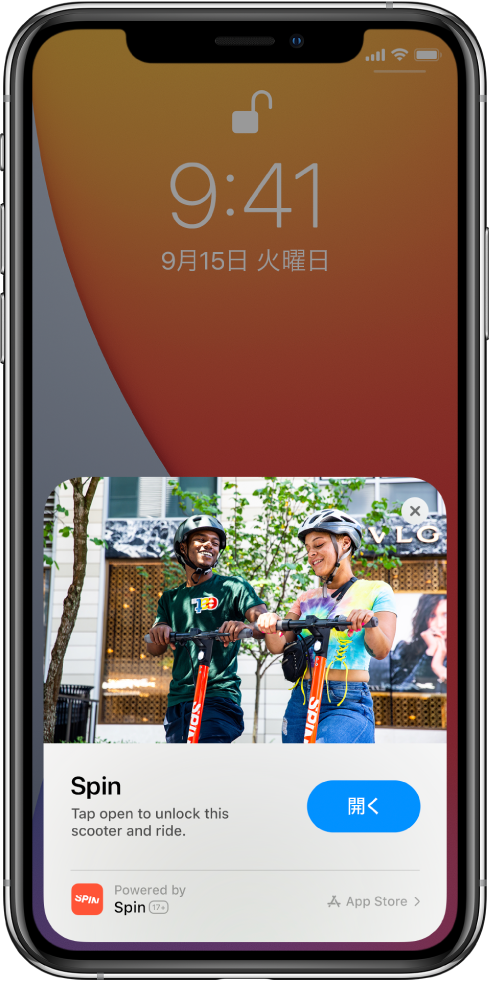
\includegraphics[height=90mm]{images/appClips.png}
  \caption{App Clips} \label{fig:appClips}
\end{figure}

\section{NFCを用いて情報を取得し、ナビゲーションに応用する研究}
NFC技術を自己位置推定やコンテキスト情報取得などに利用し、ナビゲーションに役立てている研究を紹介する。

\subsection{Bridging physical and virtual worlds with electronic tags}
WantらはBridging physical and virtual worlds with electronic tags\cite{10.1145/302979.303111}でRFIDを利用し実世界とコンピュータ世界の情報を結びつけるシステムを提案している。
このシステムでは実世界の文書や図書、カードなどにRFIDタグを設置し、これらを専用のリーダーで読み込むことで、関連した情報やURLを推薦したり他のオブジェクトとの関連を示す事ができるようになっている。

ARでの表示は行っていないが、本研究同様にNFCタグをとリーダーを利用してコンテキスト情報を取得しそれに合わせた内容を推薦するシステムである。
この研究からもNFCタグの利用はコンテキスト情報の埋め込みに置いて様々な利用が可能である事がわかる。


\subsection{GoldFish}
増井らによるGoldFish\cite{10.1145/2407696.2407699}はNFCリーダーを搭載したAndroid端末で「実世界GUI」を開発するためのJavaScriptフレームワークである。
Android端末に搭載されたNFCリーダーと加速度センサを用いて実世界に設置されたNFCタグを読み込むことで任意のプログラムを実行できるようになっている。
実行するプログラムはweb上で作成しそのURLをGoldFishに登録するため、ユーザは機能ごとにアプリをインストールする必要ないため汎用性が非常に高い。

GoldFishも本研究同様にNFCタグを実世界のコンテキストの取得に利用している研究である。
またweb上にプログラムを配置し汎用性を高めるという手法は、本研究がARのコンテツをすべてweb上にwikiのプロジェクトとして管理し、ナビゲーションのコンテキストをアプリ側で規定しない点と発想を同じくするものである。

\subsection{Development of an Indoor Navigation System Using NFC Technology}
OzdenizciらはDevelopment of an Indoor Navigation System Using NFC Technology\cite{5954491}でNFCタグを利用した室内ナビゲーションのプロトタイプ「NFC Internal」を作成している。
このプロトタイプはNFCタグにタッチすることでユーザの現在地や向きを把握し、その情報と事前に導入した地図情報から2Dマップでの経路を提示するシステムである。(図\ref{fig:NFC_Internal})

本研究同様、施設内の各所に位置情報の書かれた近距離通信のNFCタグを設置し、タグにタッチされるたびにユーザの場所と向きを更新している。
また屋内での位置測位に近距離通信のNFCタグを利用することの利点としてコストが少ない点、正確な位置と向きの情報が得られる点、通信の応答時間が短い点などを挙げており、これらは本研究が主張するNFCタグの採用理由の一部と一致する。
一方でユーザへの情報提示が2Dの地図とテキストベースであることと、何度もタグにタッチすることで目的地へ最短でたどり着くことに主眼をおいている点が本研究大きく異なると言える。

\begin{figure}[h]
  \centering 
  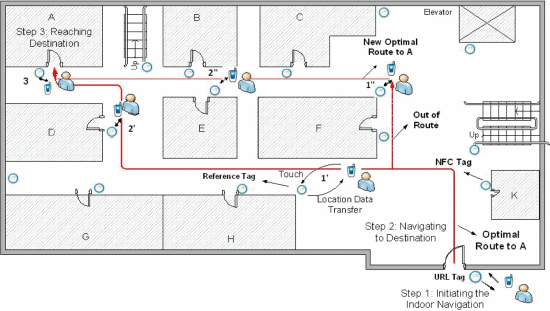
\includegraphics[width=150mm]{images/NFC_Internal.png}
  \caption{NFC Internalのイメージ} \label{fig:NFC_Internal}
\end{figure}



\section{AR・VR情報の整理・関連情報推薦にハイパーリンクを利用する研究}
ARやVRでの情報を整理するためにハイパーリンクを利用すた研究やプロジェクトを紹介する。
またハイパーリンク情報によってARとVRをシームレスに統合したシステムについても紹介する。



\subsection{VAnnotatoR}
Mehlerらが提案したVAnnotatoR\cite{10.1145/3209542.3209572}はVR/ARでのテキストや画像などのメディアをハイパーリンクを用いて管理し可視化するフレームワークである。
図\ref{fig:VAnnotatoR}のように文書や画像の他に3Dモデルや位置情報同士を関連付け、3Dでそのつながりを可視化する。
さらにユーザの入力によって表示を変えたり関連付けられた場所ワープするような探索機能を備える。

VannotatoRはホロコーストに関連する資料を整理し、可視化することで歴史を解説するStolperwegeプロジェクトが発端となっている。そのため様々な形式の資料と位置情報を互いに関連づけた上でわかりやすく可視化・ナビゲートすることに主眼をおいている。
よってハイパーリンクを利用してARで表示する情報を管理し、それら利用して関連情報を提示するという点で本研究と設計が近いが以下の点で異なっている。
\begin{itemize} 
  \item ハイパーリンク情報の編集環境に関してwikiのような誰でも入力可能なシステムを導入していない
  \item ARの表示における位置推定は考慮に入れていない
  \item HypAR Touchでは文字情報でのみハイパーリンクを形成する
\end{itemize}

\begin{figure}[h]
  \centering 
  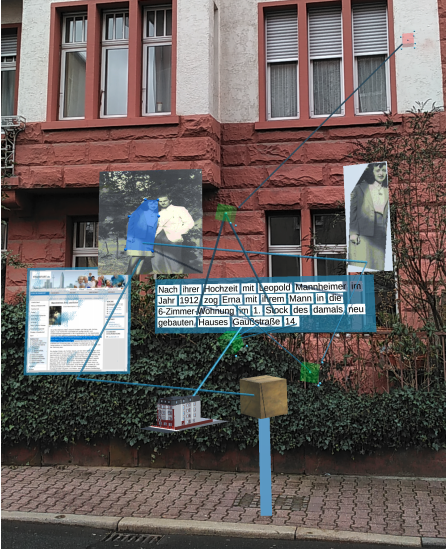
\includegraphics[height=90mm]{images/VAnnotatoR.png}
  \caption{VAnnotatoRでのAR表示} \label{fig:VAnnotatoR}
\end{figure}

\subsection{HyperReal}
RomeroらによるHyperRealは\cite{10.1145/900051.900055}仮想現実並びに複合現実におけるハイパーメディアの設計及びその設計に基づいたプロトタイプである。
単なる文字でのハイパーリンクだけでなく様々なメディアをリンクし、ユーザの遷移記録を保存し再現する機能を有するなど複雑なハイパーメディアの構築を行っている。
またプロトタイプでは博物館の案内アプリケーションを作成しており、ARで大まかな情報提示(図\ref{fig:HyperReal_ar})を行った上で詳細を仮想空間で補足する(図図\ref{fig:HyperReal_vr})ようなインターフェースを備えている。
このアイデアは本研究におけるAR情報付近へのワープ機能と類似が見られる。
一方で本研究のようにARで提示する情報の編集環境などには重点を置いておらず、あくまでも時間などを含めた複雑なハイパーメディアの構築に主眼をおいた研究である。
\begin{figure}[h]
  \centering 
  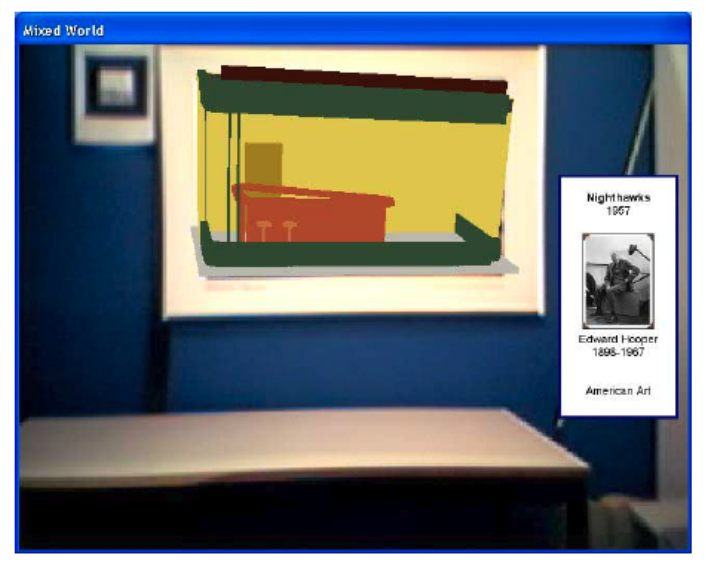
\includegraphics[height=80mm]{images/HyperReal_ar.png}
  \caption{HyperRealでのAR表示} \label{fig:HyperReal_ar}
\end{figure}

\begin{figure}[h]
  \centering 
  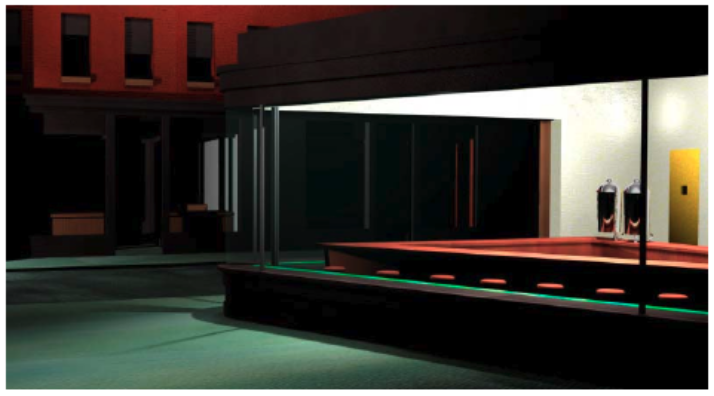
\includegraphics[height=80mm]{images/HyperReal_vr.png}
  \caption{HyperRealでのVR表示} \label{fig:HyperReal_vr}
\end{figure}


\subsection{Annotation authoring in collaborative 3D virtual environments}
小林らによるAnnotation authoring in collaborative 3D virtual environments\cite{10.1145/1152399.1152452}では、Kayらが主導した仮想OSプロジェクトCroquet\cite{10.5555/1009376.1009395}でを拡張したアノテーションシステムを提案している。
具体的には以下のような機能をもつ注釈システムを提案している。
\begin{itemize} 
  \item 特定のシーン内に注釈をつけそれらをあらゆるシーンからシーンから参照できるようにする
  \item 追加された注釈をオブジェクトとして空間上に配置しまとめることができる
  \item 注釈をフィルタするためのシステム「Interactor」を作成
  \item 注釈の変化を可視化する
\end{itemize}
これらの機能のうち、追加された注釈をオブジェクトとして空間上に配置しまとめることができる点は第\ref{link_enum_notatio}節の「リンクを利用した柔軟な記法」と類似が見られる。
表示するもののフィルタに関しても本研究での課題と言える。
一方で本研究ではAR/VRで表示する情報とその他のwikiページを等価に扱ったリンク構造を採用しており。この研究とは大きく異なると言える。

\subsection{MagicBook}
BillinghurstらによるMagicBook\cite{10.1145/634067.634087}ははARとVRの間のシームレスな移行を可能にするシステムのプロトタイプである。
Magicbookでは実際の本を利用し、本にマーカーを埋め込むことでヘッドマウントディスプレイからの自由な視点を持ったARを提供する。
さらにARで表示された状態でハンドルのスイッチを押すとシームレスにVRに移行し、自由に仮想空間状を移動することが可能になる(図\ref{fig:MagicBook})。
MagicBookのARのビューからVRへとシームレスに切り替えることでより詳細な情報を表示するという考えは本システムの移動機能に類似点が見られる。
一方で、本研究での移動はあくまでも場所から場所への移動による探索を主眼としているに対し、MagicBookは1つのAR情報を更に細くする形でVRを展開しているという点で用途に異なりがあるといえる。


\begin{figure}[h]
  \centering 
  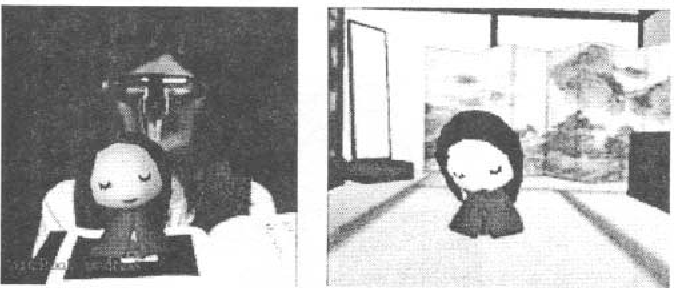
\includegraphics[width=120mm]{images/MagicBook.png}
  \caption{MagicBookでのAR(左)とVR(右)} \label{fig:MagicBook}
\end{figure}


